\subsection{Limit $\Theta_\star \to \infty$}

\begin{frame}	
	\frametitle{The limit $\Theta_\star \to \infty$}

		\begin{figure}
   			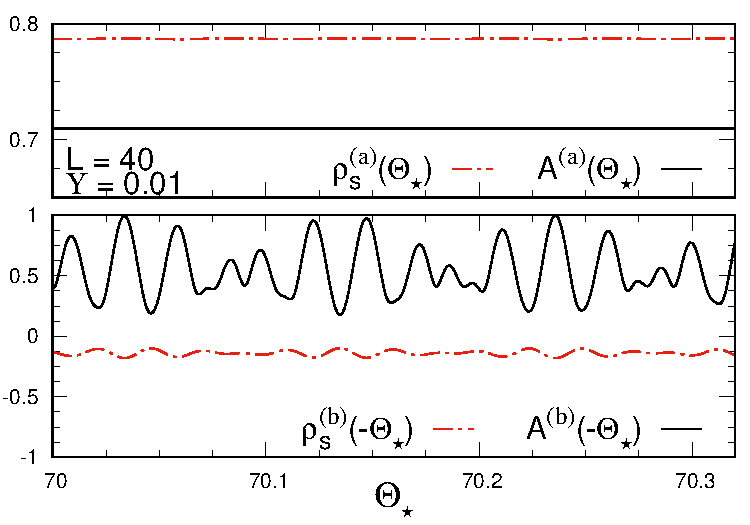
\includegraphics[width=8.4cm]{paper/diffThstaru001T70l40.pdf}
  			\caption{ {\bf Kitaev} - Fixed $L = 40$, $\Upsilon = 0.01$ versus
    			$\Theta_\star$, close to $\Theta_\star = 70$.  The top plot shows 
    			the
    			values at $\Theta=\Theta_\star$, while the bottom
    			 at $\Theta=-\Theta_\star$. }
			\label{roundtripDiffThetaAR}
		\end{figure}

	%\end{column}
	%\end{columns}
\end{frame}

\begin{comment}
	\begin{columns}
	
	\begin{column}{0.52\textwidth}
		\begin{figure}[!htb]
			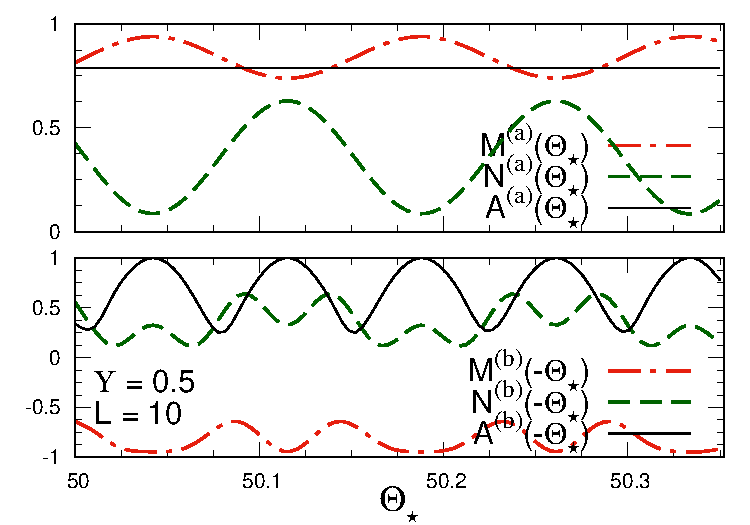
\includegraphics[width=1\columnwidth]{paper/diffThstaru50s50l10.pdf}
 			\caption{ {\bf Ising} - Fixed $L = 10$, $\Upsilon = 0.5$ versus $
 			\Theta_\star$,
 			 close to $\Theta_\star = 50$. The top plot shows the values at 
 			 $\Theta=\Theta_\star$, while the bottom plot the values 		
 			 at $\Theta=-\Theta_\star$. }
			\label{roundtripDiffTheta}
		\end{figure}
	\end{column}
\end{comment}
	%\begin{column}{0.5\textwidth}


\section{Two-Level Model}

\begin{frame}
	
	\frametitle{Two-Level Model:	$\qquad \qquad H_{2\ell}(t) = - \beta(t) 
				\sigma^{(3)}+ {\Delta\over 2} \sigma^{(1)}$}
	
	\begin{columns}
	\begin{column}{0.52\textwidth}
		\begin{figure}[!htb]
  			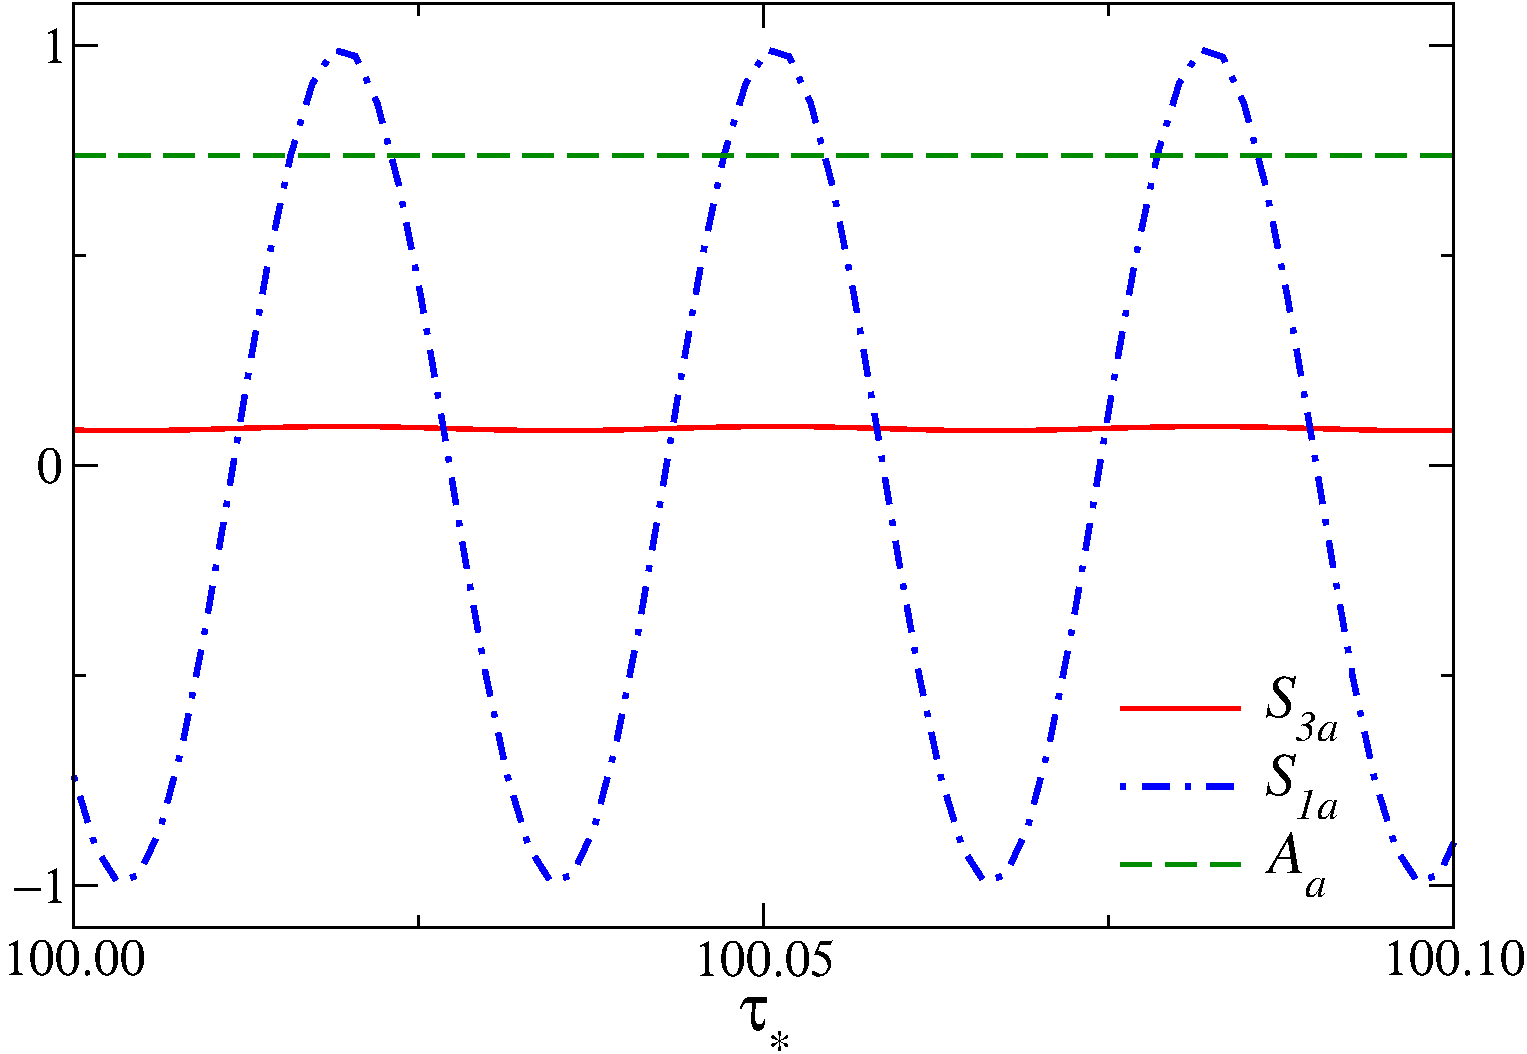
\includegraphics[width=1\columnwidth]{paper/oscillationa.pdf}
  			\caption{Dependence on $\tau_\star\equiv t_\star/\sqrt{t_s}$ at 
  			the end of the first dynamic branch for $\upsilon=1$, 
  			and $\tau_\star\approx 100$.}
 		 	\label{lzfigs}
		\end{figure}
	
	\end{column}
	\begin{column}{0.5\textwidth}
		\begin{figure}[!htb]
			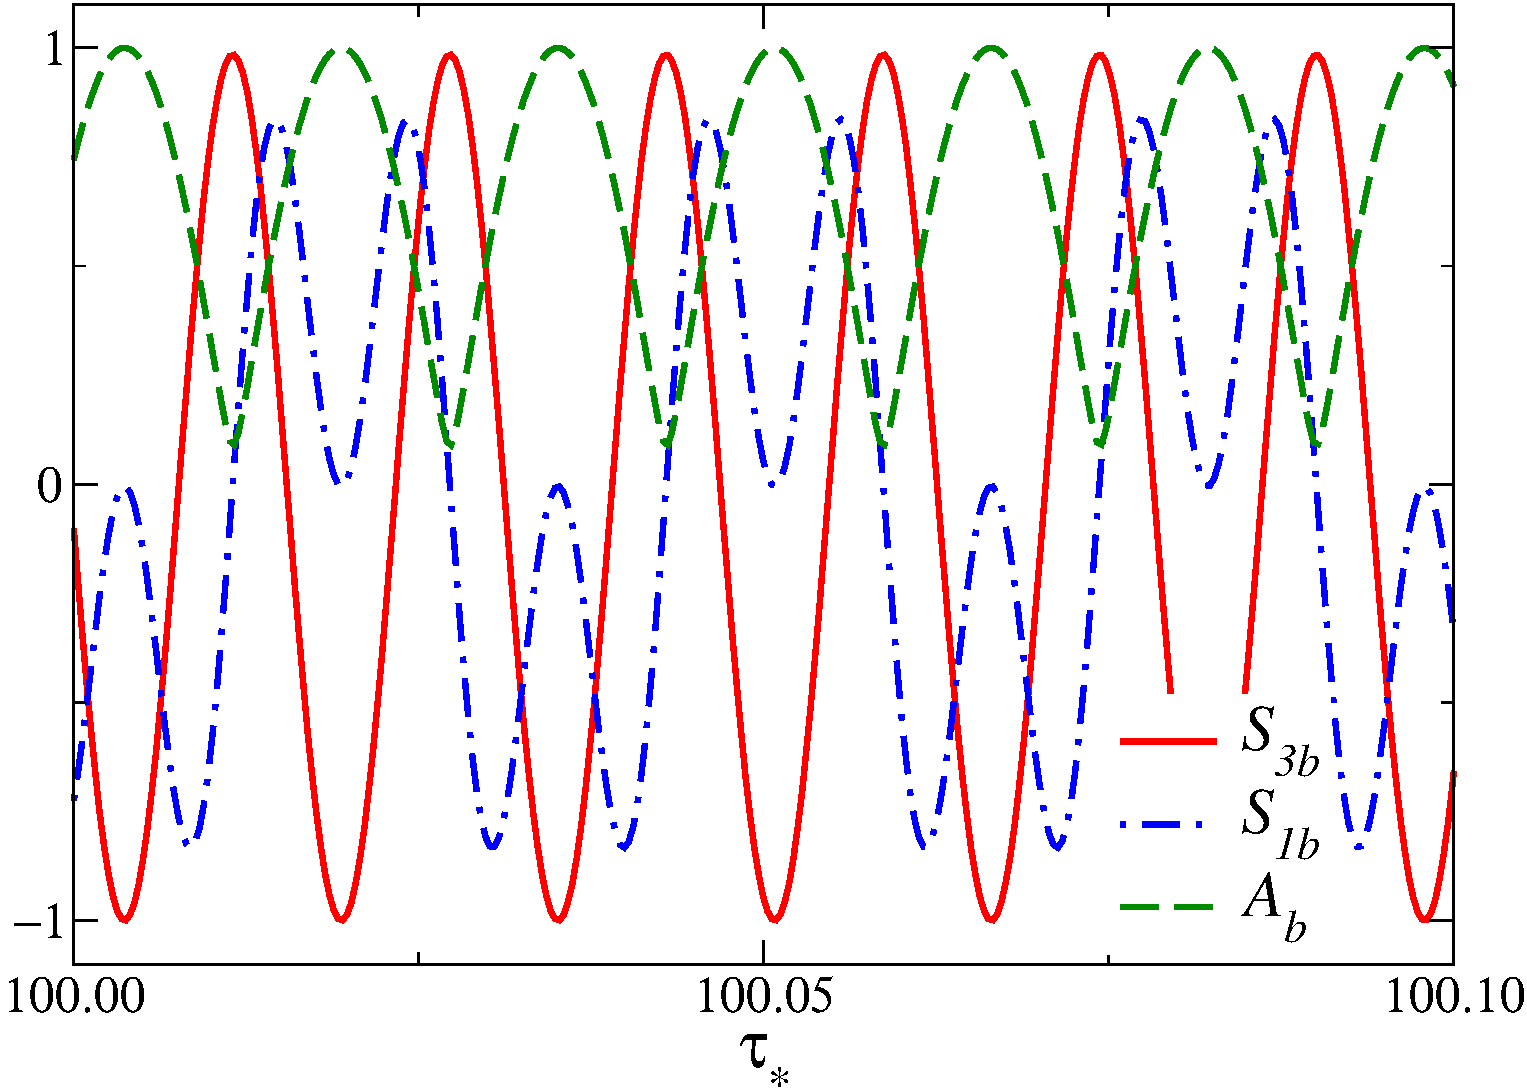
\includegraphics[width=1\columnwidth]{paper/oscillationc.pdf}
  			\caption{Dependence on $\tau_\star$ at the end of round-trip 
  			protocol for $\upsilon= t_s \Delta^2 =1$, and 
  			$\tau_\star\approx 100$.}
  			\label{lzfigs}
		\end{figure}


	\end{column}
	\end{columns}


\end{frame}
